%%%%%%%%%%%%%%%%%%%%%%%%%%%%%%%%%%%%%%%%%%%%%%%%%%%%%%%%%%%%%%%%%%%%%%%%%%%%


\documentclass[draft]{agujournal2019}
\usepackage{url} 
%\usepackage{lineno}
%\usepackage[inline]{trackchanges} %for better track changes. finalnew option will compile document with changes incorporated.
\usepackage{soul}
\usepackage{lscape}
\usepackage{adjustbox}
\usepackage{float}
\usepackage{amsmath}
\usepackage{amssymb}
\usepackage{amsthm}
\usepackage{physics}
\usepackage{setspace}
\usepackage{fix-cm}


\usepackage{graphicx}

\usepackage{wrapfig}
\usepackage{blindtext}
%Table-related commands
\usepackage{array}
%\setlength{\arrayrulewidth}{1mm}
%\setlength{\tabcolsep}{18pt}
%\renewcommand{\arraystretch}{1.5}
%\newcolumntype{s}{>{\columncolor[HTML]{AAACED}} p{3cm}}
% %-------------------------------------------------------


% defined commands
\newcommand{\unit}[1]{\ensuremath{\, \mathrm{#1}}}
% "Colored Marker" commands: wrap text in, e.g., \red{...} to highlight that color
\newcommand{\red}[1]{\textcolor{red}{#1}}
\newcommand{\blue}[1]{\textcolor{blue}{#1}}
\newcommand{\purple}[1]{\textcolor{purple}{#1}}
\newcommand{\avg}[1]{\left\langle #1 \right\rangle}
\newcommand{\vel}[0]{\mathbf{u}}
\newcommand{\B}[0]{\mathbf{B}}

%uncomment this for single-spaced version
\draftfalse

\begin{document}
\SetSinglespace{}
% preliminary title
\title{PHYS 6268: Nonlinear Dynamics, Problem Set 1}

% I defaulted to alphabetical last name, no preference here
\authors{C. Michael Haynes\affil{1}}

\affiliation{1}{School of Earth and Atmospheric Sciences, Georgia Institute of Technology, Atlanta GA, USA\\
mhaynes@eas.gatech.edu; Ford 2118}


\section*{Strogatz Book: Problems 2.1.5, 2.2.10, 2.3.3, 2.4.2, \& 2.4.9}


\section{Problem 2.1.5}
\label{sec:p1}


\subsection{Part (a)}
\label{subsec:p1a}

\textbf{Find a mechanical system that is approximately governed by $\dot x=\sin{x}$.}
\par
To do so, I spent quite a while thinking about systems that have oscillatory behavior, motivated by the trigonometric function as $\dot x$. For such systems, it is natural to think about $x$ as an angular coordinate\footnote{Akin to, e.g., $\theta$ in cylindrical polar coordinates.}. There is a countably infinite set of fixed points $X^*\equiv\{k\pi\,|k\in\mathbb{N}_0\}$, where $x^* \in X^*$. The fixed point at $x^*=0$ is unstable, meaning that small displacements of the mechanical system from $x^*=0$ must be exacerbated in time. The fixed points at $x^*=\pm\pi$ are both stable, corresponding to a configuration of the system that is resistant to small perturbations. The tricky part is, the typical examples of oscillatory systems, like harmonic oscillators, tend to have an \emph{acceleration} ($\ddot x$) proportional to the sine of the angular displacement $\sin{x}$, rather than a \emph{velocity} $\dot x$. Hence, I considered scenarios that may introduce some term, perhaps a viscous or dampening effect, that might cancel this acceleration at higher angular displacements. This train of thought ultimately yielded the following.
\par
Consider an axisymmetric buoy that has the shape of an ellipsoid, such that the center of mass lies along the midpoint of all three axes. Assume that the buoyancy of the buoy is such that the center of mass lies exactly at the water's surface. The problem with a more typical example of a rotating bar (e.g., a falling tree) is that once again (assuming it to be thin), the torque on the bar and thus the \emph{second} derivative of the angular coordinate $x$ is proportional to $\sin{x}$: there needs to be some mechanism that begins to slow its acceleration following the inflection point of $\sin{x}$, $x=\pi/4$. In the buoy example, since a substantial fraction ($\approx1/2$) of the buoy is submerged, the accelerating rotation will be met with an enhanced hydrodynamic resistance. Since, for ``round" objects this usually is $\propto\dot x$, I take this mechanical relationship to approximately reflect the desired dynamical system, $\dot x = \sin{x}$.




\subsection{Part (b)}
\label{subsec:p1a}

\textbf{Using your physical intuition, explain why it now becomes obvious that $x^*=0$ is an unstable fixed point and $x^*=\pi$ is stable.}
\par

The stability of either configuration is revealed by envisioning such a buoy in the presence of still water, and the introduction of small surface water waves represents a small perturbation. In perfectly still water, the buoy could remain ``upright", where the semi-major axis is aligned with the gravitational force. This corresponds to the fixed point $x^*=0$. However, any small perturbation from this will ``topple" the buoy to a more stable, horizontally-aligned configuration. This is the fixed point at $x^*=\pi$. Since the water slows the rotation as the buoy is accelerated in the angular ($x$) direction, the buoy does not continue to rotate all the way to the next \emph{unstable} fixed point $x^*=2\pi$, but instead relaxes to equilibrium at $x^*=\pi$.


\newpage



\section{Problem 2.2.10}
\label{sec:p2}
\textbf{For each of (a)-(e), find an equation $\dot x = f(x)$ with the stated properties, or if there are no examples, explain why not. (In all cases, we assume that $f(x)$ is smooth, and that $x\in\mathbb{R}$).}


\subsection{(a) Every real number is a fixed point}
\label{subsec:p2a}
$\dot x = f(x) = 0$


\subsection{(b) Every integer is a fixed point, and there are no others}
\label{subsec:p2b}
$\dot x = f(x) = \sin{(\pi x)}$


\subsection{(c) There are precisely three fixed points, and all of them are stable.}
\label{subsec:p2c}
This is \textbf{not possible} to construct (at least restricted to one-dimensional, real-valued dynamical systems). The stability of the fixed point $x^*$ is determined by the sign of the derivative $\textrm{sgn}({\dot x^*})$ on either side of $x^*$. A fixed point is stable, or a \emph{sink}, when the derivative is positive for smaller $x$ values and negative for larger values of $x$. For two consecutive fixed points to be classified as stable, then the derivative would have to point ``toward" \emph{both} points simultaneously: due to the intermediate value theorem, this implies the derivative passes through zero, creating another fixed point. Otherwise, the derivative $f$ would have to change signs \emph{without} passing through another fixed point, requiring $f$ to possess a jump discontinuity. Such a step violates the smoothness criterion that was established in the prompt, and hence, it is not possible to have a function $f$ with three separate, stable fixed points. 


\subsection{(d) There are no fixed points.}
\label{subsec:p2d}
$\dot x = f(x) = r$ such that $r \in \{\mathbb{R}/\{0\}\}$. For example, $f(x) = 2 \qquad \forall x$.


\subsection{(e) There are precisely 100 fixed points.}
\label{subsec:p2e}

To construct a function $\dot x = f(x)$ that has exactly 100 fixed points, we employ a 100$^\mathrm{th}$ degree polynomial since it can possess up to 100 intersections where $f=0$. Such a polynomial $f(x)$ would look like:
\begin{equation*}
    f(x) \in \mathbb{P}_{(100)}(x) \longrightarrow \sum_{n=0}^{100} a_n x^n \qquad .
\end{equation*}
An immediate consequence of the fundamental theorem of algebra guarantees that a degree $n$ polynomial possesses $n$ roots in the complex plane, a slightly weaker condition than what $f$ must achieve to ensure 100 distinct fixed points. To satisfy the conditions, $f$ must only include real, un-repeated roots. A procedure utilizing Sturm's Theorem and treatment of polynomial roots can construct a general requirement for the coefficients $a_n$ to guarantee $n$ real, un-repeated roots. 
\par
Similar to some of the previous parts, this is satisfied for an infinite family of functions that obey these criteria. One example is ${f(x) = \Pi_{n=0}^{100} (x^n - n)}$. 




\newpage



\section{Problem 2.3.3}
\label{sec:p3}


\textbf{The growth of cancerous tumors can be modeled by the Gompertz law $\dot N = -a N \ln{(b N)}$, where $N(t)$ is proportional to the number of cells in the tumor, and $a,b>0$ are parameters.}

\subsection{Part (a)}
\label{subsec:p3a}
\textbf{Interpret $a$ and $b$ biologically.}
\par
$a$: This parameter corresponds to the ``loss rate" of the tumor. A large $a$ corresponds to a more quickly decaying population, for given values of $N,N_0$.

$b:$ This parameter corresponds to the ``carrying capacity" of the tumor. At large $t$, the tumor concentration will approach a constant value that corresponds to $b$. 


\subsection{Part (b)}
\label{subsec:p3b}
The expression 
\begin{equation*}
    \dot N = \frac{\mathrm{d}N}{\mathrm{d}t} = -a N \ln{bN}
\end{equation*}
is separable, so we integrate:
\begin{equation*}
    \int_{N_0}^N \frac{\mathrm{d}N}{N \ln{bN}} = -a\int_0^t \mathrm{d}t \qquad .
\end{equation*}
\begin{equation*}
    \implies\ln\left(\frac{\ln{bN}}{\ln{bN_0}}\right) = -a\,t \qquad ,
\end{equation*}
which simplifies to an expression for $N(t)$, 
\begin{equation}
\label{eqn:1}
    N(t) = \frac{(b N_0)^{e^{-at}}}{b} \qquad .
\end{equation}

\begin{figure}
    \centering
    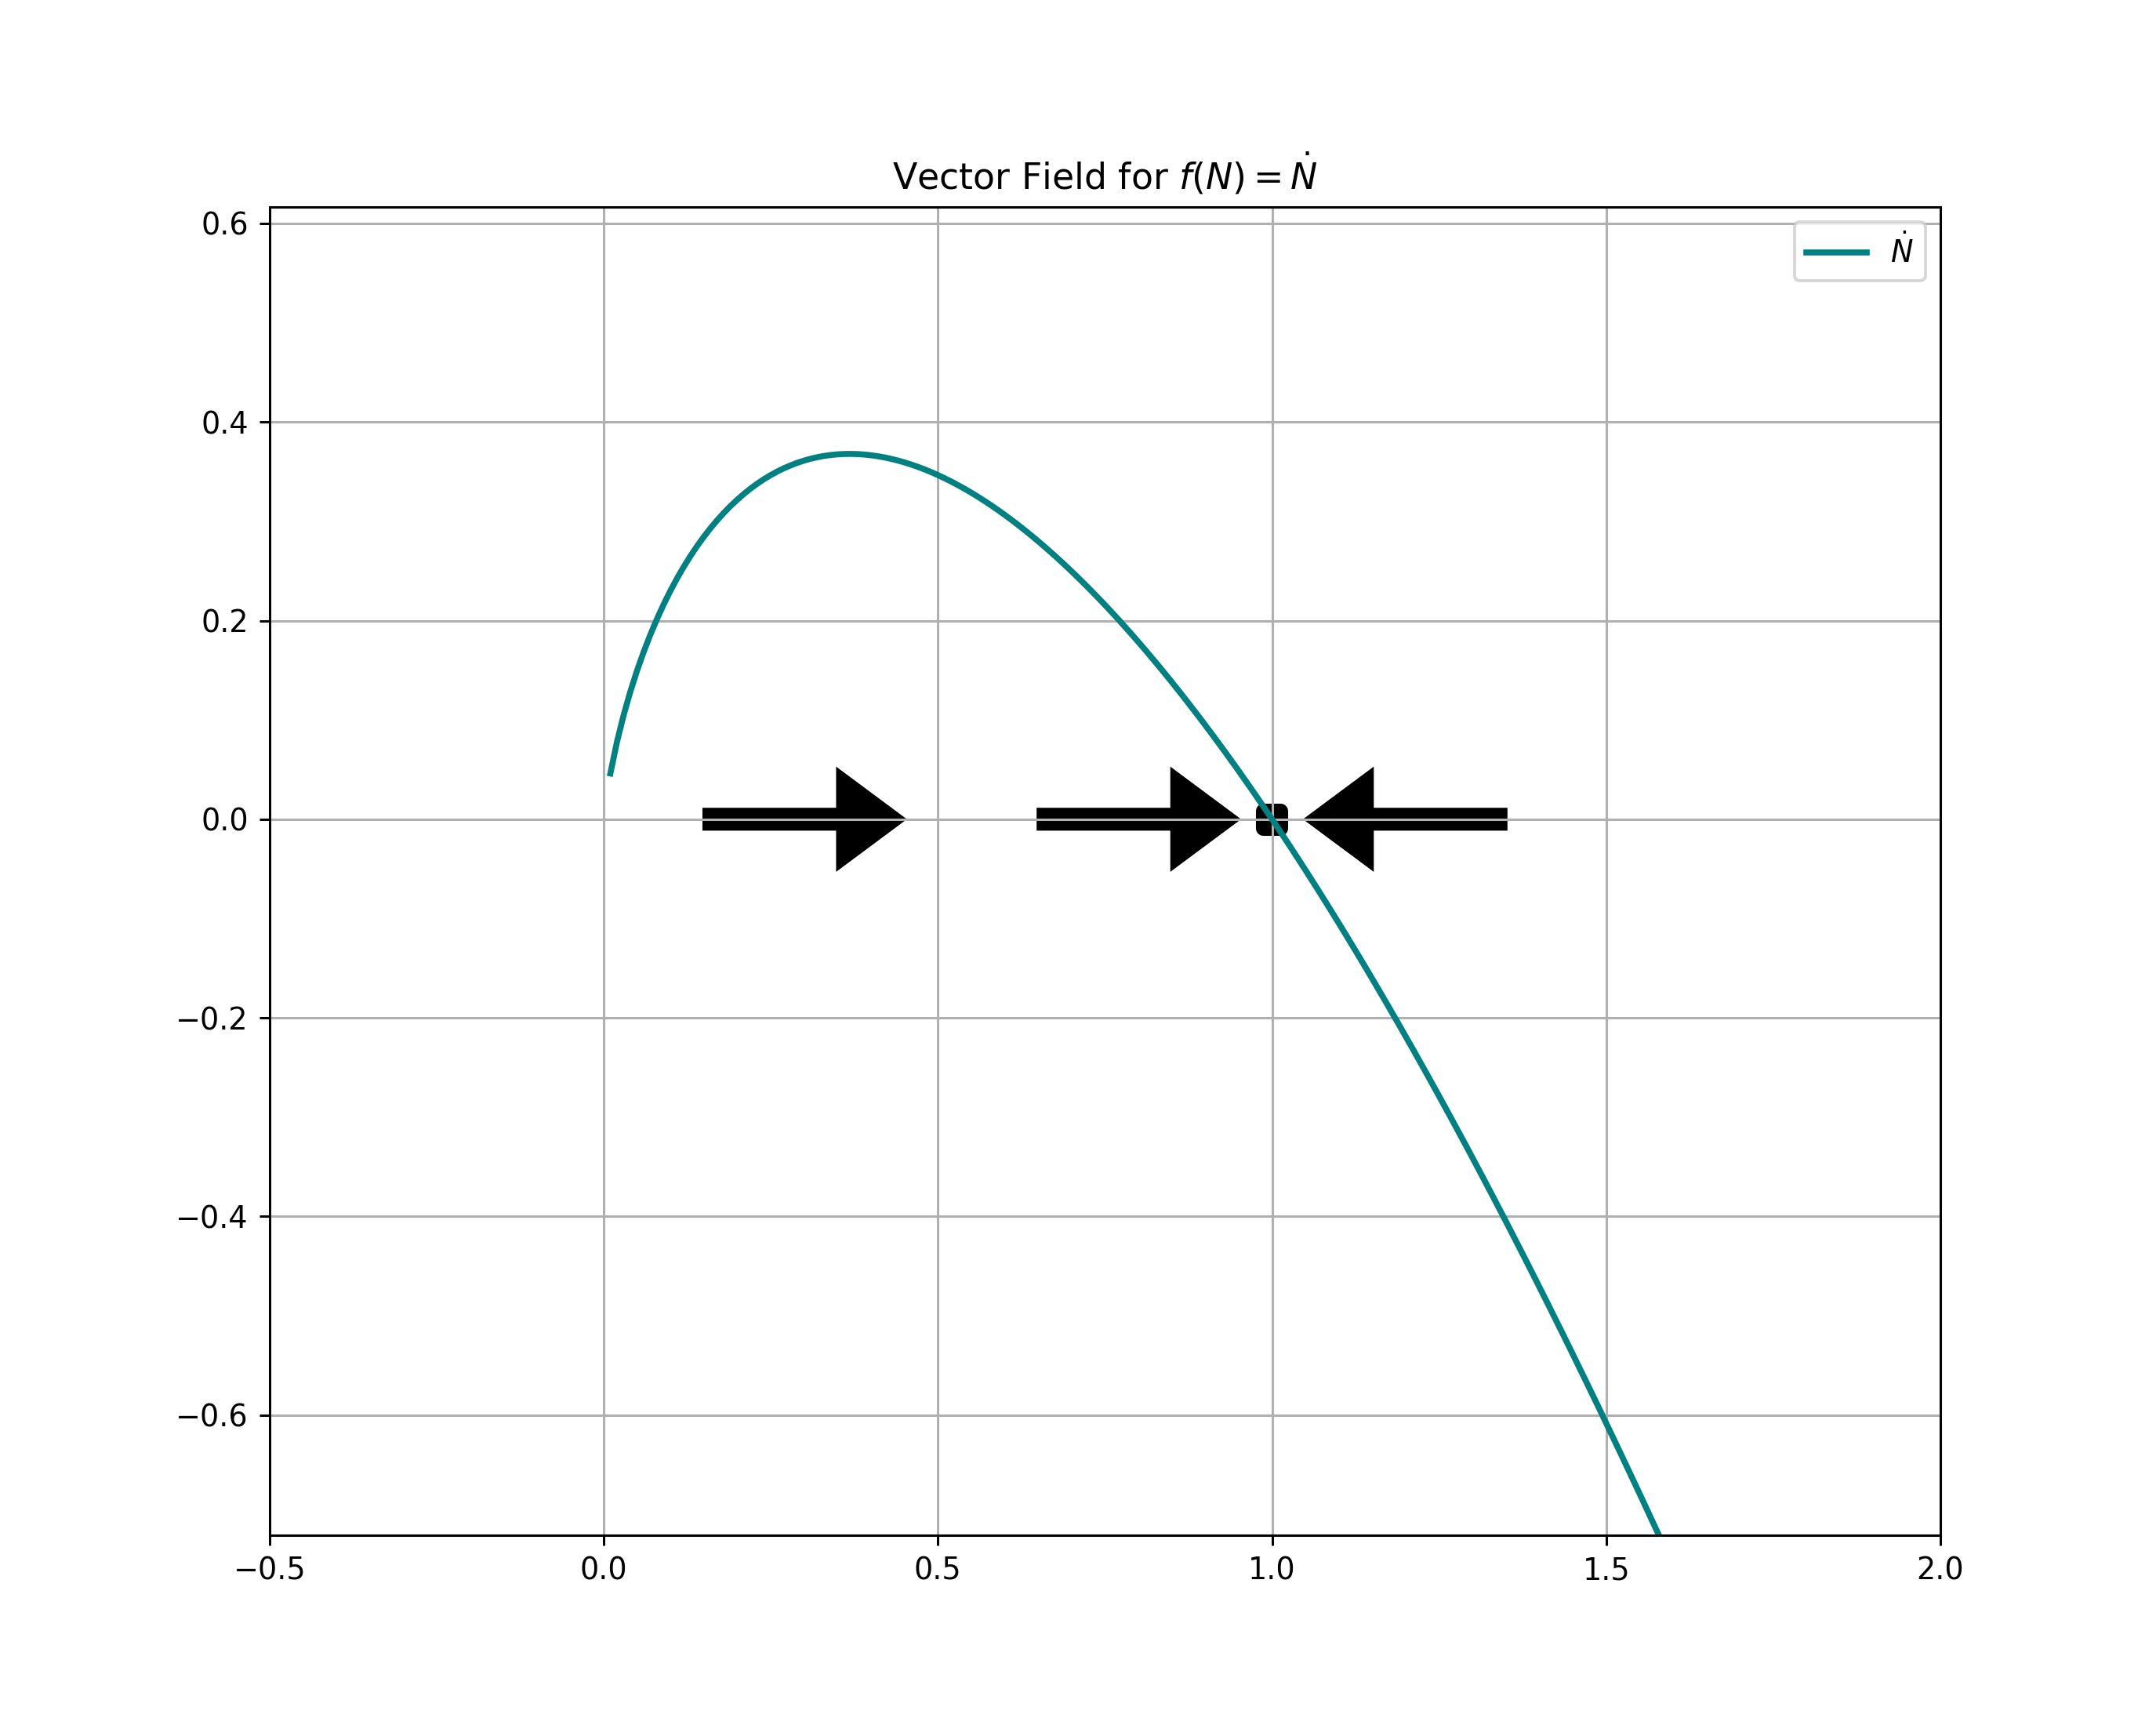
\includegraphics[width=0.65\linewidth]{figures/1D_vector_field_f.png}
    \caption{Vector field of $f(N) = \dot N$, for constants $a=b=1$. The arrows indicate the direction of the flow, and the black point marks a stable fixed point of $\dot N$. An unstable fixed point is located at the origin.}
    \label{fig:1}
\end{figure}

The plots of $\dot N$ and $N(t)$ are included in Figures \ref{fig:1} and \ref{fig:2}, respectively.


\begin{figure}
    \centering
    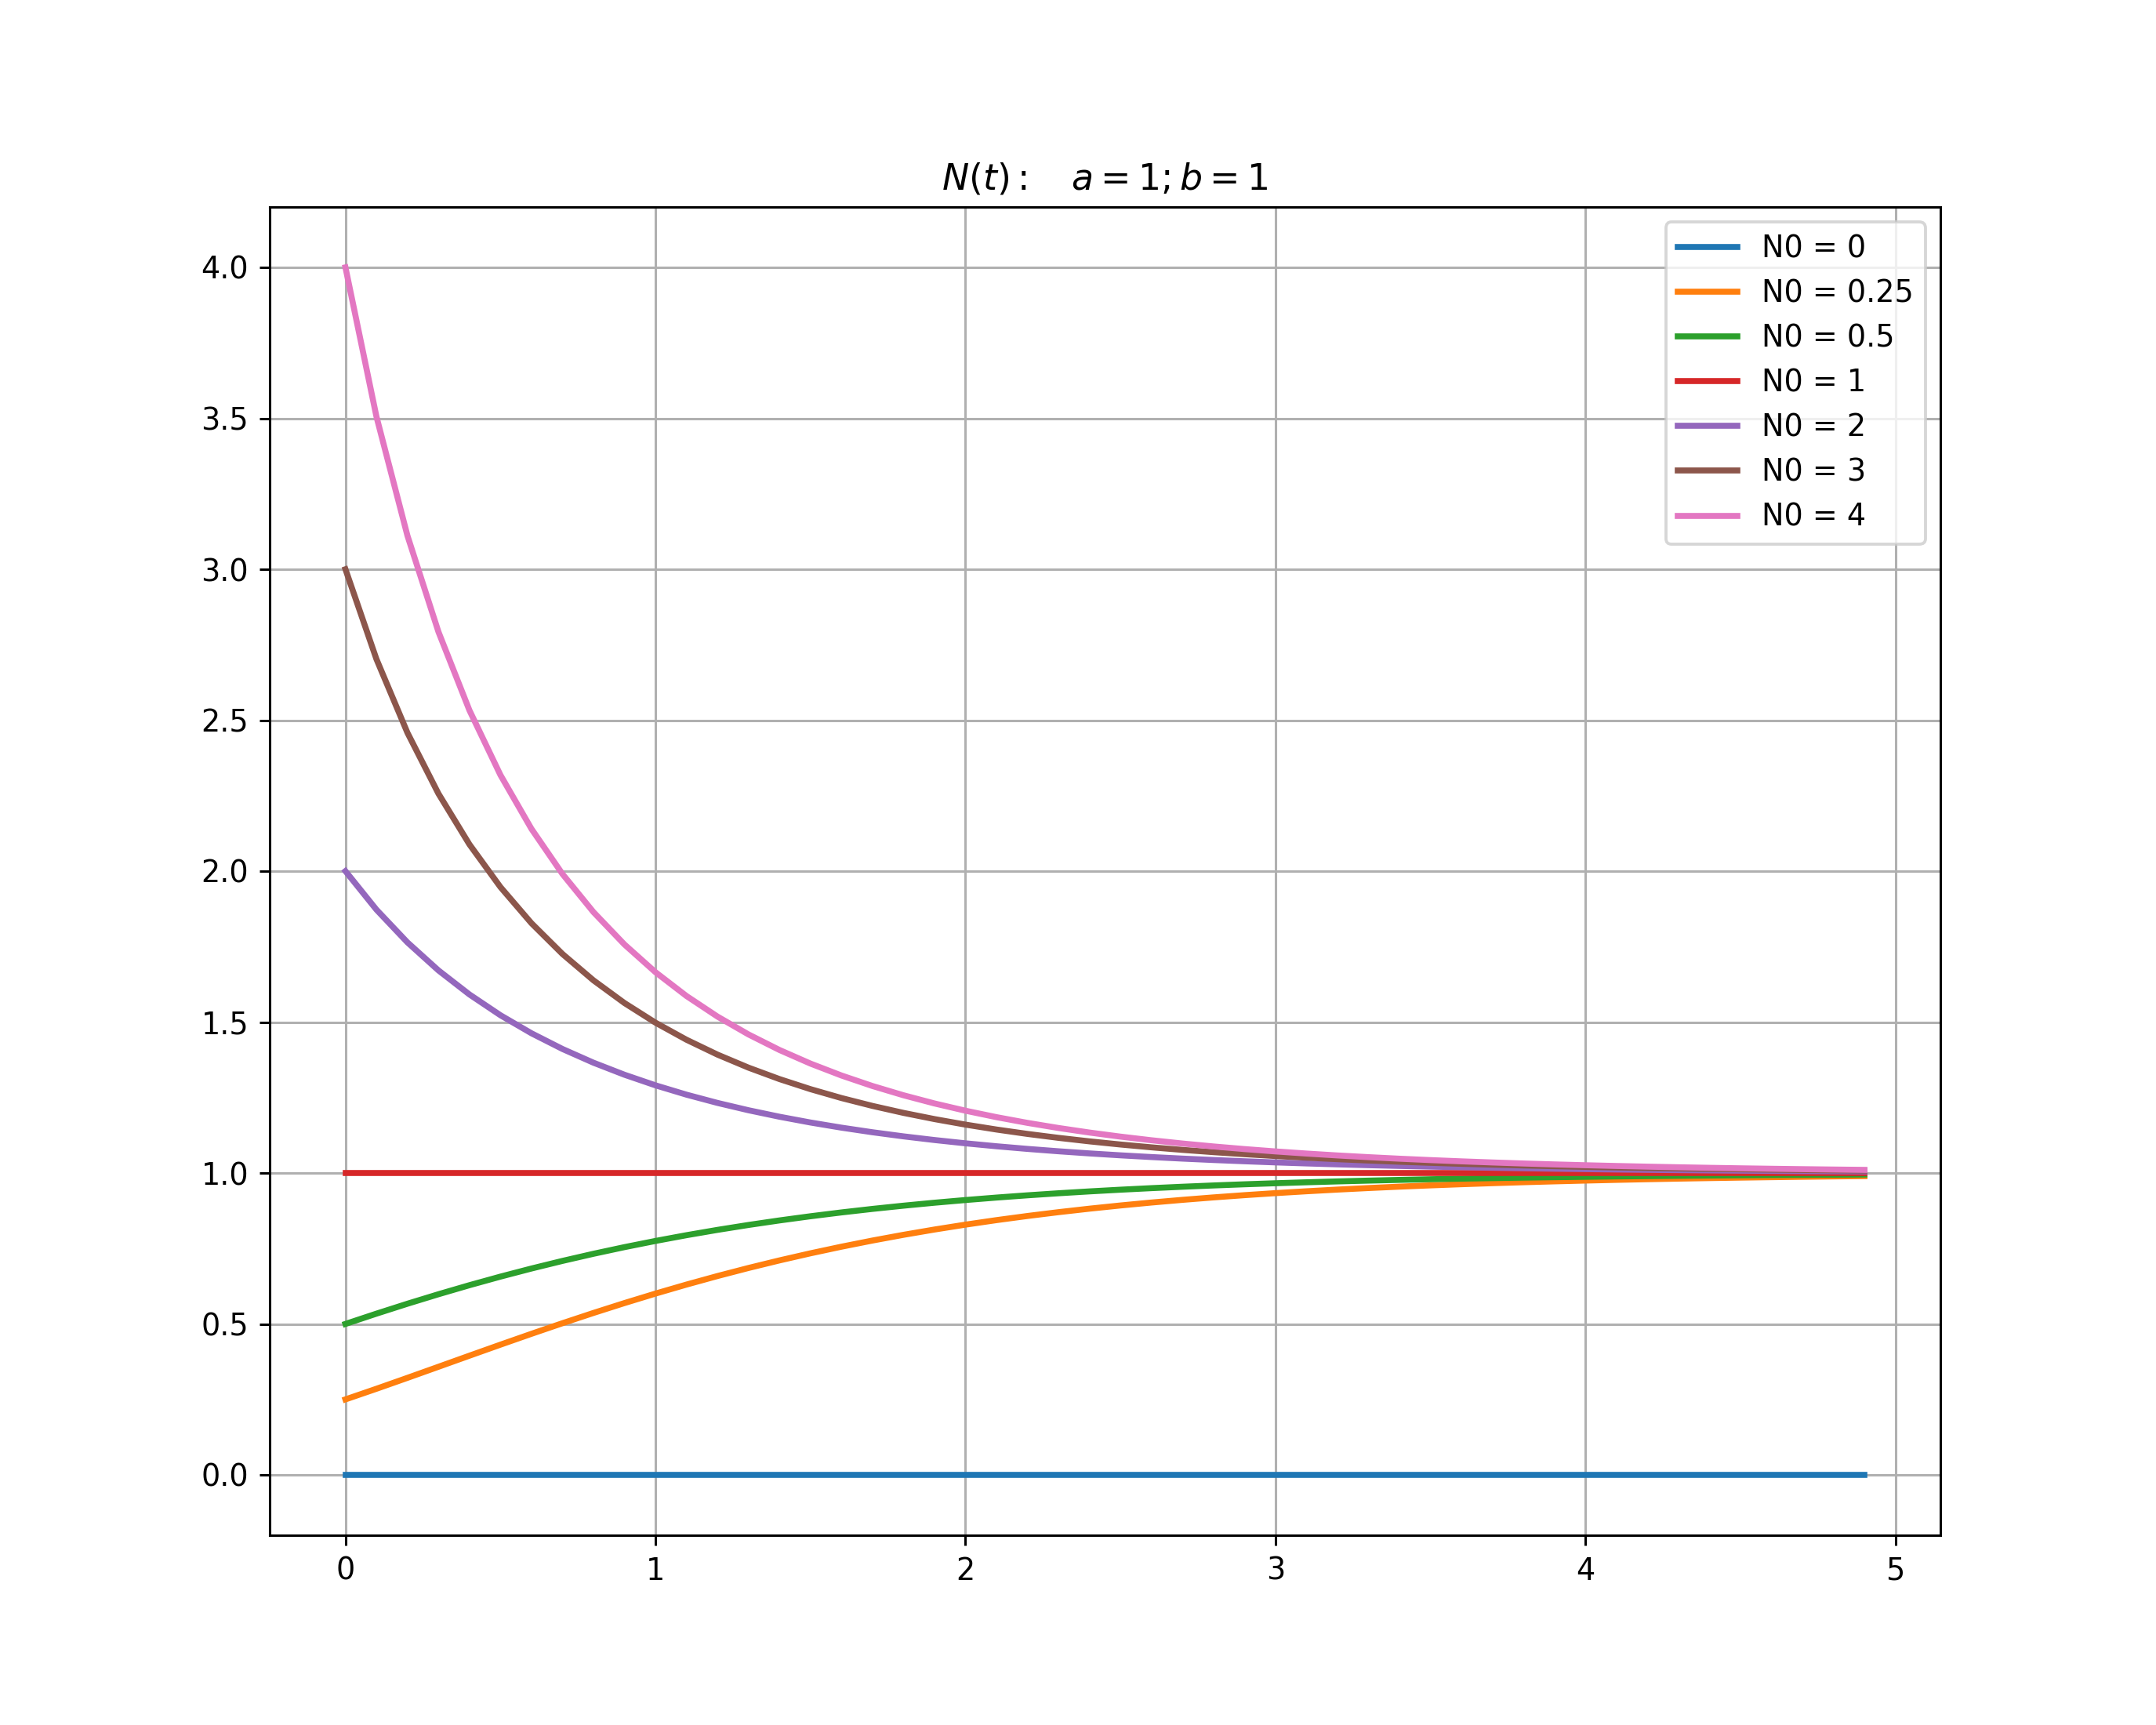
\includegraphics[width=1.\linewidth]{figures/plot_Ns.png}
    \caption{Plots of various $N(t)$ curves (see equation (\ref{eqn:1}). $N(t)$ is visualized for different initial conditions (see Figure label). The coefficients are given by $a=b=1$ to generate these curves, consistent with the derivative $\dot N$ shown in Figure \ref{fig:1}. }
    \label{fig:2}
\end{figure}

\newpage


\section{Problem 2.4.2}
\label{sec:p4}
\textbf{Use linear stability analysis to classify the fixed points of the following system:}
\begin{equation*}
    \dot x = x(1-x)(2-x) \qquad .
\end{equation*}

Linear stability analysis involves evaluating the derivative of the flow $f'$ at the locations of the fixed points $x^*$. The sign of the derivative corresponds to the stability: if $f'(x^*)<0$, then $x^*$ is stable. If $f'(x^*)>0$, then $x^*$ is unstable. This analytical correspondence is equivalent to the graphical approach used in Figure \ref{fig:1}. Furthermore, the magnitude of $f'$ corresponds to a characteristic timescale $1/{|f'(x^*)|}$ of the convergence or divergence. 
\par

For this expression, the fixed points lie at $f(x^*)=0 \implies x^*\in\{0,1,2\}$. Differentiating $\dot x = f(x)$ w.r.t. $x$ yields $f'(x)=3x^2 - 6x + 2$. Evaluating $f'(x^*)$ yields the following:
\begin{align}
    x^* = 0: \quad f'(x*) = 2, \quad\longrightarrow \mathrm{unstable} \\
    x^* = 1: \quad f'(x*) = -1, \quad\longrightarrow \mathrm{stable} \\
    x^* = 2: \quad f'(x*) = 2, \quad\longrightarrow \mathrm{unstable} \qquad .
\end{align}

\newpage


\section{Problem 2.4.9}
\label{sec:p5}
\textbf{In statistical mechanics, the phenomenon of ``critical slowing down" is a signature of a second-order phase transition. At the transition, the system relaxes to equilibrium much more slowly than usual. Here's a mathematical version of that effect:}

\subsection{Part (a)}
\label{subsec:p5a}
\textbf{Obtain an analytical solution to $\dot x = -x^3$ for an arbitrary initial condition. Show that $x(t)\longrightarrow0$ as $t\longrightarrow\infty$, but that the decay is not exponential. }

We begin with
\begin{equation*}
    \dot x = \frac{\mathrm{d}x}{\mathrm{d}t} = -x^3 \qquad ,
\end{equation*}
which is readily separable:
\begin{equation*}
    \frac{\mathrm{d}x}{x^3} = - \mathrm{d}t \qquad .
\end{equation*}
Integration yields 
\begin{equation*}
    2 t = x^{-2} - x_0^{-2} \implies x^2 = \frac{1}{2t + \frac{1}{x_0^2}} \qquad .
\end{equation*}
We have introduced $x_0$ to represent the initial data of the system. This produces two solutions, along the positive and negative branches, given by
\begin{equation}
\label{eqn:sol5a}
    x(t) = \pm \frac{1}{\sqrt{2t + \frac{1}{x_0^2}}} \qquad .
\end{equation}
To determine asymptotic behavior for large $t$, we evaluate the limit (of the positive branch):
\begin{equation*}
    \lim_{t\longrightarrow\infty} x(t) = \lim_{t\longrightarrow\infty} \frac{1}{\sqrt{2t + \frac{1}{x_0^2}}} \simeq \lim_{t\longrightarrow\infty} \frac{1}{\sqrt{2t}} = \frac{1}{\infty} = 0 \qquad .
\end{equation*}
Hence, we have shown that $x(t)\longrightarrow 0$ as $t\longrightarrow\infty$ for an arbitrary initial condition ($x_0$). The decay follows $1/\sqrt{2t}$, which is asymptotically slower than $e^-t$ which vanishes more rapidly with increasing $t$. 


\subsection{Part (b)}
\label{subsec:p5b}
\textbf{To get some intuition about the slowness of the decay, make a numerically accurate plot of the solution for the initial condition $x_0=10$, for $t\in[0,10]$. Then, on the same graph, plot the solution to $\dot x = -x$ for the same initial condition. }
\par
To begin, we obtain a solution for the comparison through separation and integration:
\begin{equation*}
    \dot x = -x \implies \frac{\mathrm{d}x}{x} = -\mathrm{d}t \implies \ln{\frac{x}{x_0}} = -t \qquad .
\end{equation*}
Exponentiation yields the solution $x(t)$:
\begin{equation}
\label{eqn:sol5b}
    x(t) = x_0 e^{-t} \qquad .
\end{equation}
Figure \ref{fig:3} shows the requested curves, equations (\ref{eqn:sol5a}) and (\ref{eqn:sol5b}).
As depicted in the figure, the system from part (a; see section \ref{subsec:p5a}) tends much less rapidly to $x(t)\approx0$ than the exponentially decaying system in comparison.

\begin{figure}[t]
    \centering
    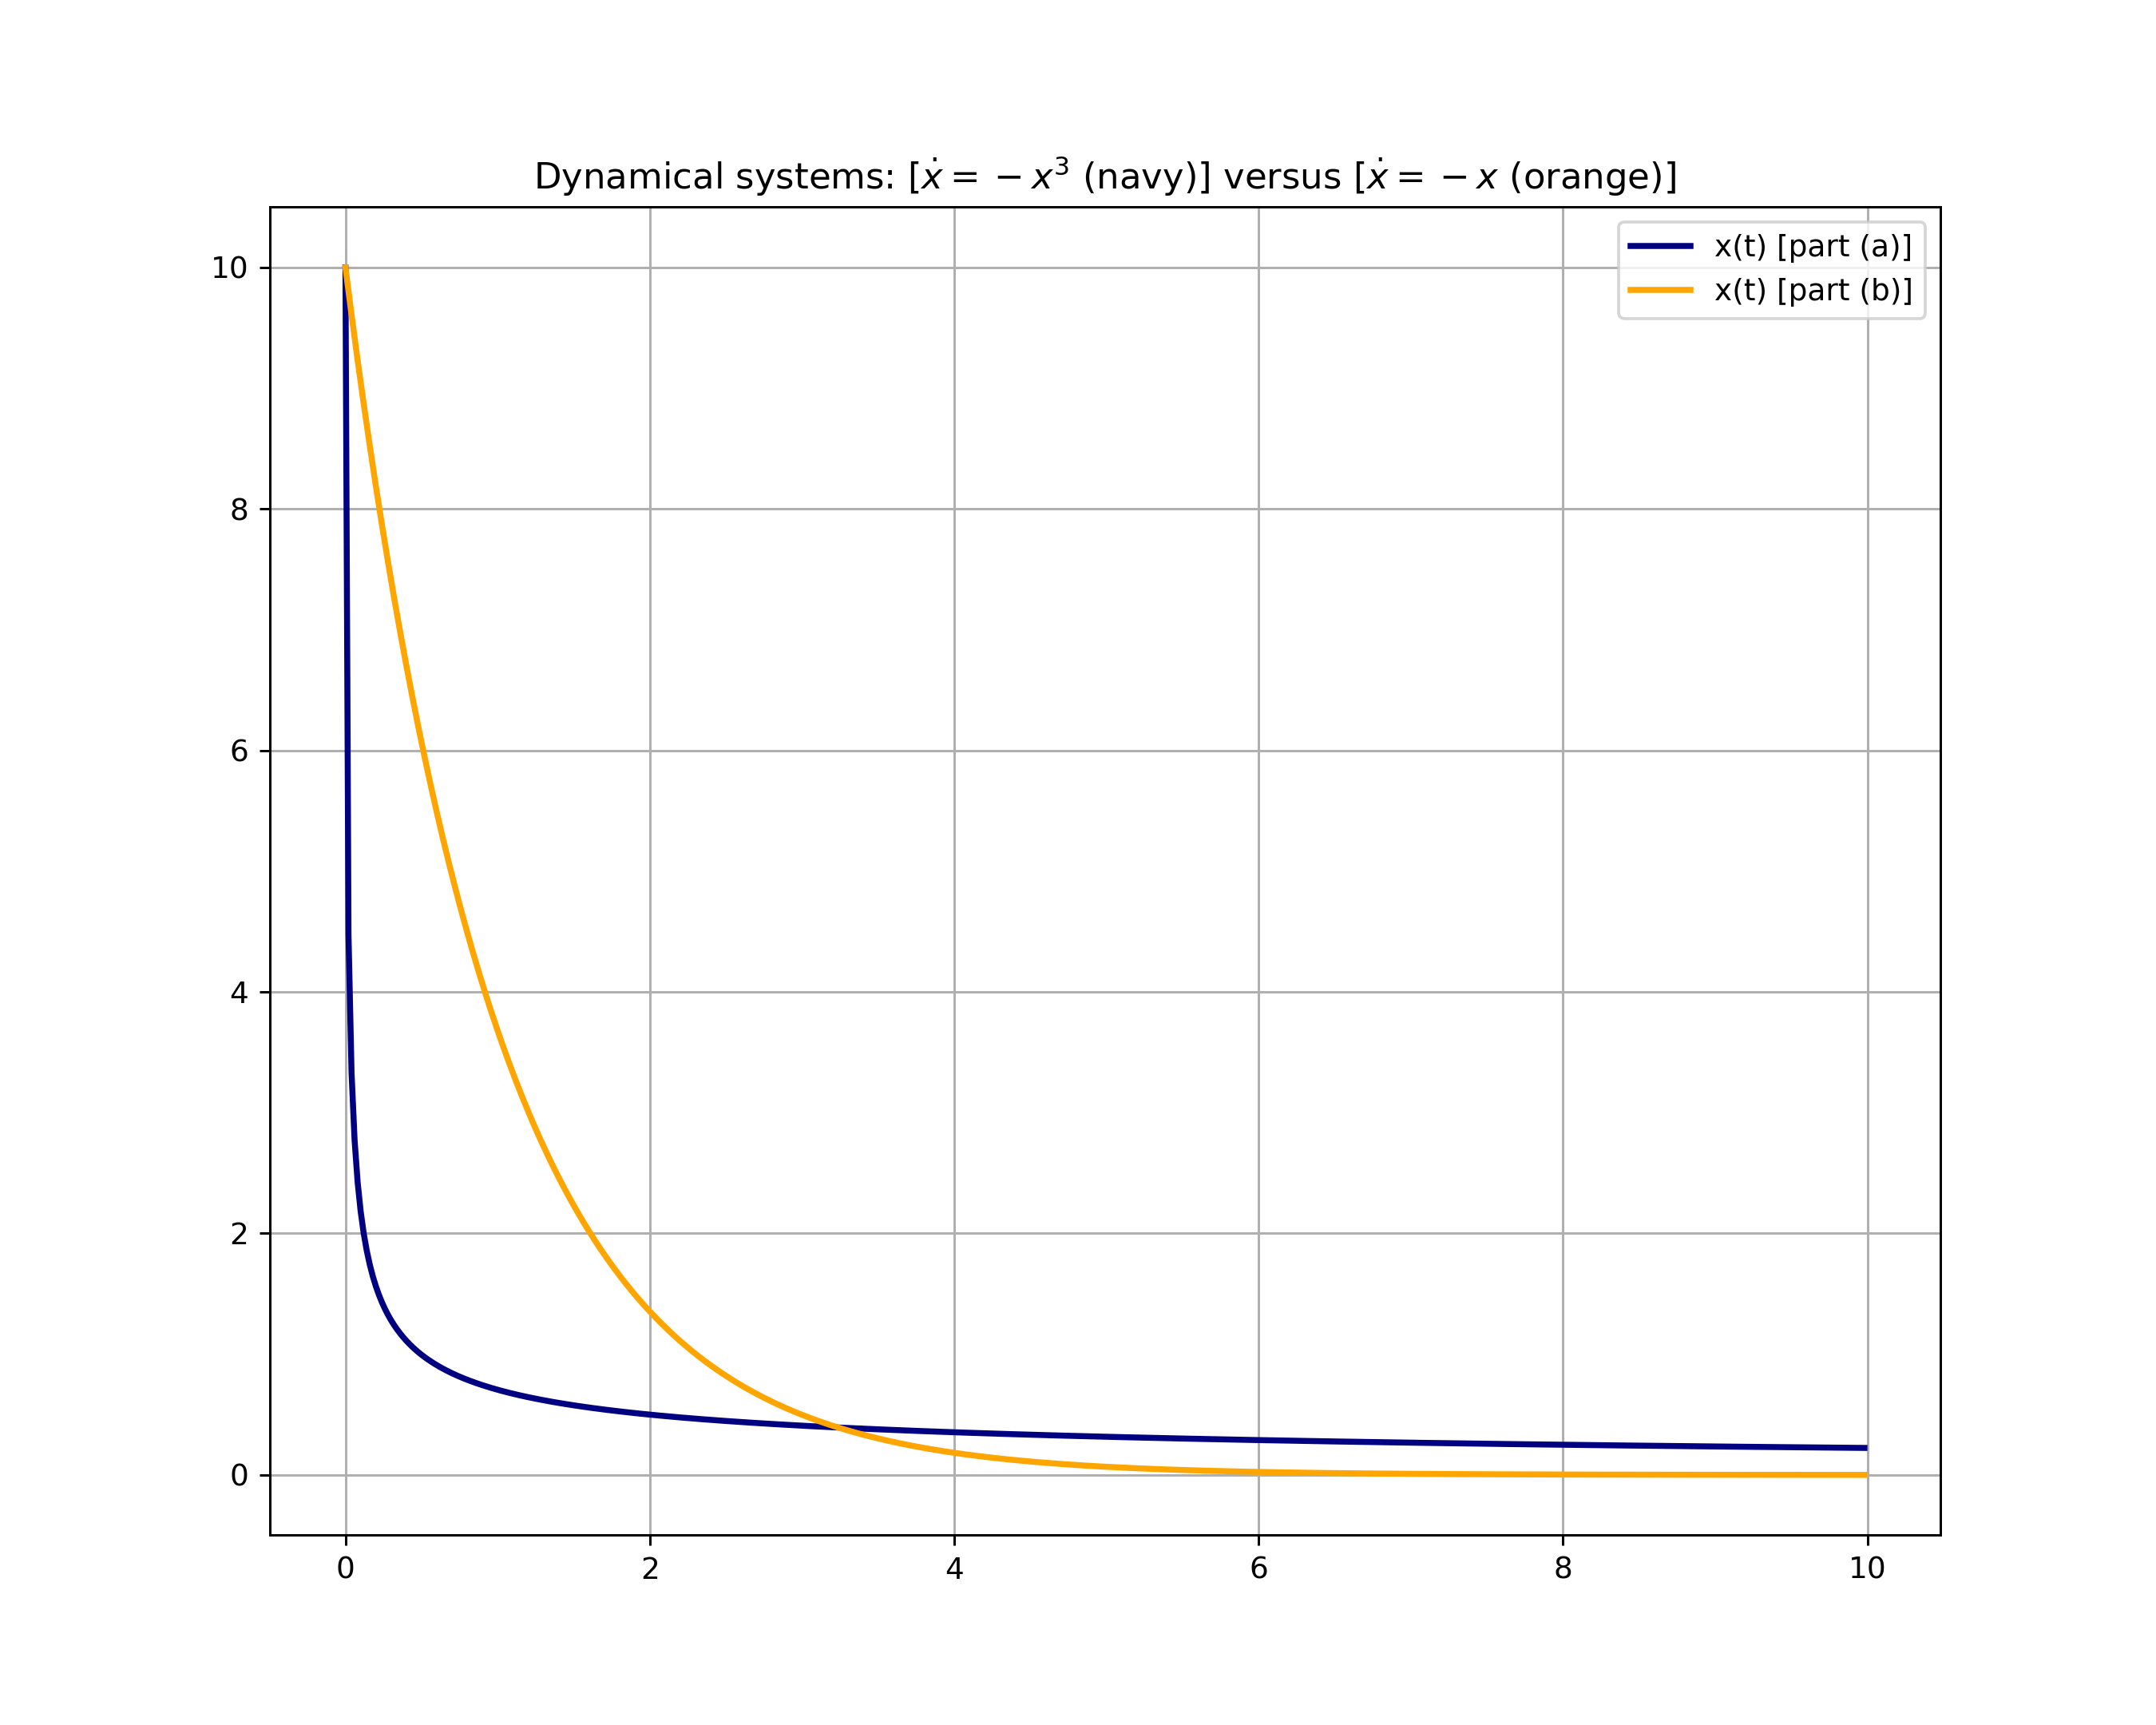
\includegraphics[width=0.85\linewidth]{figures/plot_xt.png}
    \caption{Plots of $x(t)$ trajectories for different dynamical systems. The navy curve represents a solution to equation (\ref{eqn:sol5a}), and the orange curve is a solution to equation (\ref{eqn:sol5b}). Both have an initial condition of $x_0=10$, indicated by their first intersection. }
    \label{fig:3}
\end{figure}



\section{Software Usage}
The entirety of the work was carried out on pen and paper prior to typesetting, except for the plotting: this was completed using python (\verb|matplotlib|). 

%\section{Acknowledgments}
\newpage














%%%%%%%%%%%%%%%%%%%%%%%%%%%%%%%%%%%%%%%%%%%%%%%
% \newpage
% \clearpage

%\bibliography{MHD}
\end{document}
